\documentclass[11pt]{article}

\usepackage[margin=1.04in]{geometry}
\usepackage[T1]{fontenc}
\usepackage{amsmath}
\usepackage{amssymb}
\usepackage{array}
\usepackage{booktabs}
\usepackage{caption}
\usepackage{float}
\usepackage{graphicx}
\usepackage{microtype}
\usepackage{url}
\usepackage[section]{placeins}
\usepackage{tikz}
\usetikzlibrary{arrows.meta,positioning}

\captionsetup{labelsep=period,font=small}
\setlength{\parindent}{0pt}
\setlength{\parskip}{0.55em}
\renewcommand{\arraystretch}{1.08}

\DeclareMathOperator{\CVaR}{CVaR}
\newcommand{\Dc}{D^{c}}
\newcommand{\De}{D^{e}}
\newcommand{\Da}{D^{a}}
\newcommand{\ind}{\mathbf{1}}

\title{\vspace{-3.0em}Validation Study for Direct CVaR-CJE\vspace{-0.9em}}
\author{}
\date{}

\begin{document}
\maketitle
\vspace{-2.0em}

This is a validation note for the lower-tail score CVaR extension of Direct
Mean-CJE. The original Direct Mean-CJE estimator used
a cheap judge score to predict an oracle score. The CVaR extension keeps that
spirit but changes the prediction target: for each possible cutoff, it predicts
the oracle shortfall below that cutoff (tail risk). At the very end, we add a section that estimates CVaR on the Arena dataset. 

\section{Known Data Generating Process}

Throughout this study we use this known data generating process. The outcome is an oracle score \(Y\) between zero and one.  The cheap judge score
\(S\) is a noisy monotone signal of \(Y\).  Each policy shape has its own Beta
distribution for \(Y\).
\[
  Y_p \sim \operatorname{Beta}(a_p,b_p),
  \qquad
  S_p = 4(Y_p-0.5)+\varepsilon,
  \qquad
  \varepsilon \sim N(0,0.8^2).
\]
For a lower-tail level \(\alpha\), let \(q_{\alpha,p}\) be the \(\alpha\)
quantile of \(Y_p\).  The target is
\[
  v_{\alpha,p}
  =
  \frac{1}{\alpha}
  \int_0^{q_{\alpha,p}} y\,dF_p(y).
\]

\begin{figure}[H]
\centering
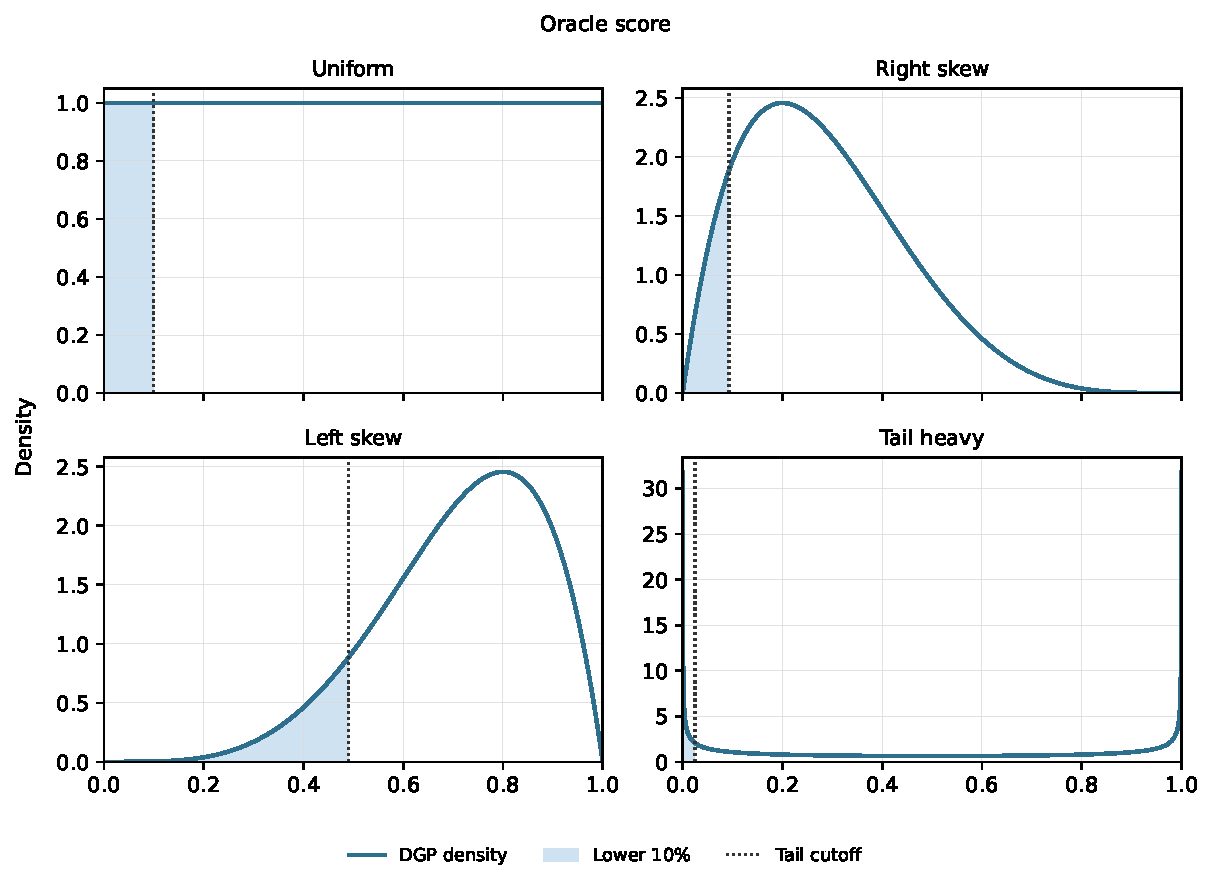
\includegraphics[width=0.88\linewidth]{figures/dgp_policy_distributions.pdf}
\caption{Four known outcome distributions.  The shaded area is the lower ten percent of outcomes.}
\label{fig-dgp}
\end{figure}

At \(\alpha=0.10\), this lower-tail score CVaR is the average oracle score in
the worst ten percent of the policy distribution.
This validation DGP is continuous, so there is no probability mass exactly at
the cutoff.  In discrete settings, the target truth calculation splits any atom
at the selected quantile so that exactly an \(\alpha\) share of the distribution
enters the lower tail.

\begin{table}[H]
\centering
\small
\begin{tabular}{@{}lrrrrr@{}}
\toprule
Policy shape & Truth \(N\) & \(a\) & \(b\) & Mean & CVaR 10\% \\
\midrule
Uniform & \(\infty\) & 1.0 & 1.0 & 0.5000 & 0.0500 \\
Right skew & \(\infty\) & 2.0 & 5.0 & 0.2857 & 0.0597 \\
Left skew & \(\infty\) & 5.0 & 2.0 & 0.7143 & 0.4000 \\
Tail heavy & \(\infty\) & 0.5 & 0.5 & 0.5000 & 0.0082 \\
\bottomrule
\end{tabular}
\caption{Known ground truth for the four policy shapes.}
\label{tab-truth}
\end{table}

\subsection{Three samples: Calibration, Evaluation, and Audit}

It is important to distinguish between three \textit{non-overlapping} samples.  The \textit{calibration sample} \(\Dc\)
has cheap judge scores and expensive oracle labels; it is used to fit
cutoff-specific shortfall models \(\hat h_t(s)\), not a single model for the
oracle score.  The \textit{evaluation sample} \(\De\), is a large sample generated under the target policy distribution, has
cheap judge scores but no oracle labels; it uses those shortfall models to estimate the target policy tail
value \textit{in the absence of real oracle labels}. The \textit{transport audit sample} \(\Da\), is a smaller sample generated under target policy distribution, has oracle labels
and is used only to check whether the fitted shortfall relationship still applies. 

\begin{figure}[H]
\centering
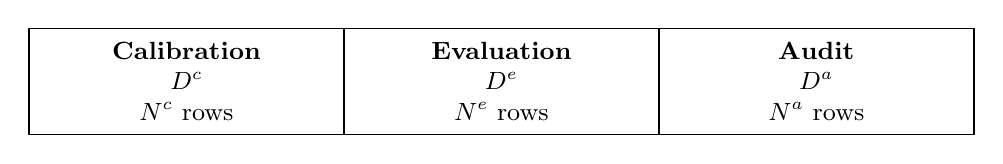
\begin{tikzpicture}[
  segment/.style={align=center, font=\small, text width=3.80cm},
  guide/.style={draw=black, line width=0.5pt}
]
\draw[guide] (0,0) rectangle (12.0,1.35);
\draw[guide] (4.0,0) -- (4.0,1.35);
\draw[guide] (8.0,0) -- (8.0,1.35);
\node[segment] at (2.0,0.68) {\textbf{Calibration}\\ \(\Dc\)\\ \(N^c\) rows};
\node[segment] at (6.0,0.68) {\textbf{Evaluation}\\ \(\De\)\\ \(N^e\) rows};
\node[segment] at (10.0,0.68) {\textbf{Audit}\\ \(\Da\)\\ \(N^a\) rows};
\end{tikzpicture}
\caption{Sample split used by the validation study.}
\label{fig-split}
\end{figure}

\subsection{Logger and Target Policies}

The \textit{base} or \textit{logger} policy of $Y$ is the distribution that generates the
calibration sample.  The \textit{target} policy is the distribution that generates the
evaluation and audit samples. Throughout this study, ``same policy distribution''
means the same marginal distribution of \(Y\). Each policy-shape row is therefore its own
base-target experiment, not a comparison among policies. Later on, when we want to test the audit, we keep \(Y\) fixed but change the joint relationship between \(S\) and \(Y\). 
And at the very end when we test on Arena data, we will show both cases: one where the logger and target policies are the same, and one where they differ (closer to what the original paper does with base vs other policies).

\FloatBarrier

\section{CVaR-CJE Estimator}

Recall that the Direct Mean CJE learns how the cheap judge score \(S\) maps to the oracle score
\(Y\).  Direct CVaR-CJE needs a different target because CVaR is about the
lower tail, not the average.  For a cutoff \(t\), the relevant quantity is the
\textit{shortfall} \((t-Y)_+\): it is zero when the oracle score is above the cutoff,
and it is positive by exactly the amount the oracle score falls below the
cutoff.

The estimator searches over a tail-dense cutoff grid \(T=\{t_1,\ldots,t_m\}\).
The grid has 61 points, includes both endpoints 0 and 1, and places extra
points on \([0,0.1]\), where small-\(\alpha\) lower-tail cutoffs are most likely.
For each candidate cutoff \(t_k\), it fits a separate shortfall model on the
calibration sample.  The shortfall model is \(\hat h_{t_k}(s)\).  It predicts
shortfall below \(t_k\), not the oracle score itself.  With calibration rows
\((s_i^c,y_i^c)\), define
\[
  z_{ik}^c=(t_k-y_i^c)_+,
  \qquad
  \hat h_{t_k}(s)
  \approx
  \mathbb{E}\bigl[(t_k-Y)_+ \mid S=s\bigr].
\]
For every cutoff, the fitted model is decreasing isotonic regression of
\(z_i(t)=(t-y_i)_+\) on \(s_i\).  The same model class and the same monotonicity
constraint are used for every \(t_k\). The critical point is that each cutoff has its own fitted shortfall model
\(\hat h_{t_k}\). The model answers how much shortfall below \(t_k\) is
expected when the cheap judge score is \(s\).

After the shortfall models are fit, the evaluation sample chooses the cutoff that works best accross all these models.
For each
\(t_k\),
\[
  \hat\Psi_\alpha(t_k)
  =
  t_k
  -
  \frac{1}{\alpha N^e}
  \sum_{i=1}^{N^e} \hat h_{t_k}(s_i^e).
\]
The selected cutoff and final point estimate are
\[
  \hat t_\alpha
  =
  \arg\max_{t_k \in T}\hat\Psi_\alpha(t_k),
  \qquad
  \hat v_\alpha
  =
  \max_{t_k \in T}\hat\Psi_\alpha(t_k).
\]

\begin{figure}[htbp]
\centering
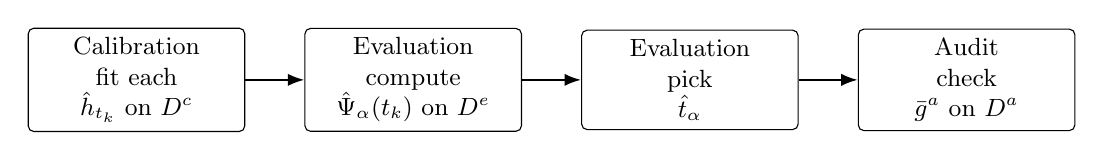
\begin{tikzpicture}[
  box/.style={draw, rounded corners=2pt, minimum width=2.75cm, minimum height=1.05cm, align=center, font=\small},
  arrow/.style={-{Latex[length=2.1mm]}, thick}
]
\node[box] (fit) {Calibration\\ fit each\\ \(\hat h_{t_k}\) on \(\Dc\)};
\node[box, right=0.75cm of fit] (score) {Evaluation\\ compute\\ \(\hat\Psi_\alpha(t_k)\) on \(\De\)};
\node[box, right=0.75cm of score] (pick) {Evaluation\\ pick\\ \(\hat t_\alpha\)};
\node[box, right=0.75cm of pick] (audit) {Audit\\ check\\ \(\bar g^a\) on \(\Da\)};
\draw[arrow] (fit) -- (score);
\draw[arrow] (score) -- (pick);
\draw[arrow] (pick) -- (audit);
\end{tikzpicture}
\caption{Estimator flow from cutoff-specific shortfall models to the audit moments.}
\label{fig-flow}
\end{figure}

\subsection{CVaR Reduces to Mean at \(\alpha=1\)}

At \(\alpha=1\), lower-tail CVaR is the mean.  Direct CVaR-CJE should then
match the corresponding mean estimator. The estimator identity matches Direct
Mean-CJE up to machine precision; Table~\ref{tab-mean} reports the resulting
estimate against the population mean.

\begin{table}[H]
\centering
\small
\begin{tabular}{@{}lrrrrrr@{}}
\toprule
Policy shape & Reps & \(N^c\) & \(N^e\) & Estimate & True mean & Difference \\
\midrule
Uniform & 60 & 499 & 1000 & 0.4987 & 0.5000 & -0.0013 \\
Right skew & 60 & 499 & 1000 & 0.2843 & 0.2857 & -0.0014 \\
Left skew & 60 & 499 & 1000 & 0.7138 & 0.7143 & -0.0005 \\
Tail heavy & 60 & 499 & 1000 & 0.5018 & 0.5000 & 0.0018 \\
\bottomrule
\end{tabular}
\caption{Mean check at \(\alpha=1\).  The average \(N^c\) is rounded.}
\label{tab-mean}
\end{table}

\section{Validation Metrics}

\subsection{Sampling Bias and Variance of the Estimator}

The validation compares repeated estimates to the known truth.  Let
\(\hat v_{\alpha,p}^{(r)}\) be the estimate for policy \(p\) in replication
\(r\), and let \(v_{\alpha,p}\) be the known value from Table~\ref{tab-truth}.
With \(R\) replications, the repeated-estimate mean and sample variance are
\[
  \bar{\hat v}_{\alpha,p}
  =
  \frac{1}{R}\sum_{r=1}^R \hat v_{\alpha,p}^{(r)},
  \qquad
  s_{\alpha,p}^2
  =
  \frac{1}{R-1}\sum_{r=1}^R
  \bigl(\hat v_{\alpha,p}^{(r)}-\bar{\hat v}_{\alpha,p}\bigr)^2.
\]
The bias, RMSE, and Monte Carlo standard error of the repeated-estimate mean
\footnote{The standard-error column is the Monte Carlo standard error of the
repeated-run mean, not the uncertainty estimate from a single fitted model.}
are
\[
  \operatorname{Bias}_{\alpha,p}
  =
  \bar{\hat v}_{\alpha,p}-v_{\alpha,p},
  \qquad
  \operatorname{RMSE}_{\alpha,p}
  =
  \sqrt{
  \frac{1}{R}\sum_{r=1}^R
  \bigl(\hat v_{\alpha,p}^{(r)}-v_{\alpha,p}\bigr)^2
  },
  \qquad
  \operatorname{SE}_{\alpha,p}
  =
  \frac{s_{\alpha,p}}{\sqrt{R}}.
\]
The estimates are computed on \(\De\) after the shortfall models are fit on
\(\Dc\).

\subsection{Selected Tail Threshold Matches Ground Truth}

We find that the the selected cutoff $t$ tracks the known ten
percent quantile for each policy shape.

\begin{table}[H]
\centering
\small
\begin{tabular}{@{}lrrrrrrr@{}}
\toprule
Policy shape & Reps & \(N^c\) & \(N^e\) & True cutoff & Mean cutoff & Bias & RMSE \\
\midrule
Uniform & 300 & 600 & 1000 & 0.1000 & 0.0990 & -0.0010 & 0.0123 \\
Right skew & 300 & 600 & 1000 & 0.0926 & 0.0918 & -0.0008 & 0.0061 \\
Left skew & 300 & 600 & 1000 & 0.4897 & 0.4906 & 0.0009 & 0.0156 \\
Tail heavy & 300 & 600 & 1000 & 0.0245 & 0.0251 & 0.0006 & 0.0056 \\
\bottomrule
\end{tabular}
\caption{Cutoff choice at \(\alpha=0.10\).}
\label{tab-cutoff}
\end{table}

\subsection{Direct CVaR-CJE Matches Known CVaR}

The estimated lower-tail value tracks the
known ten percent CVaR. The point estimator is close to the known truth in all four policy shapes.


\begin{table}[H]
\centering
\small
\begin{tabular}{@{}lrrrrrrr@{}}
\toprule
Policy shape & Reps & \(N^c\) & \(N^e\) & Estimate & True CVaR & Bias & RMSE \\
\midrule
Uniform & 300 & 600 & 1000 & 0.0505 & 0.0500 & 0.0005 & 0.0074 \\
Right skew & 300 & 600 & 1000 & 0.0595 & 0.0597 & -0.0002 & 0.0049 \\
Left skew & 300 & 600 & 1000 & 0.4005 & 0.4000 & 0.0005 & 0.0146 \\
Tail heavy & 300 & 600 & 1000 & 0.0085 & 0.0082 & 0.0003 & 0.0022 \\
\bottomrule
\end{tabular}
\caption{Direct CVaR-CJE accuracy at \(\alpha=0.10\).}
\label{tab-cvar}
\end{table}

\subsection{Estimator Comparison with Mean Plug-In Baselines}

Table~\ref{tab-method} is a diagnostic comparison with 20 replications.  Its role is to check whether the ``saddle-point form"
has lower repeated-run error than simpler mean plug-in approaches.

Table~\ref{tab-method} also shows two plug-in baselines.  The first baseline,
Mean quantile, fits the ordinary mean model
\(\hat m(s)=1-\hat h_1(s)\), sorts the evaluation predictions
\(\hat m(s_i^e)\), and averages the bottom \(\lfloor\alpha N^e\rfloor\)
values.  The second baseline, Mean dual, uses the same saddle objective as the
Direct estimator but substitutes the mean-model shortfall
\((t-\hat m(s_i^e))_+\) for the cutoff-specific shortfall model
\(\hat h_t(s_i^e)\):
\[
  \hat\Psi_{\alpha}^{\operatorname{mean\ dual}}(t)
  =
  t
  -
  \frac{1}{\alpha N^e}
  \sum_{i=1}^{N^e}(t-\hat m(s_i^e))_+.
\]
These two rows are comparison baselines, not the estimator being checked.
They are intentionally weak for lower-tail validation because they try to
estimate tail behavior from the mean model rather than learning
\(\mathbb{E}[(t-Y)_+ \mid S=s]\) directly.

\begin{table}[H]
\centering
\scriptsize
\begin{tabular}{@{}llrrrrrr@{}}
\toprule
Policy shape & Method & \(\alpha\) & Reps & \(N^c\) & \(N^e\) & Bias & RMSE \\
\midrule
Uniform & \textbf{Direct saddle point} & 0.10 & 20 & 600 & 1000 & \textbf{-0.0005} & \textbf{0.0074} \\
Uniform & Mean quantile & 0.10 & 20 & 600 & 1000 & 0.0747 & 0.0764 \\
Uniform & Mean dual & 0.10 & 20 & 600 & 1000 & 0.0741 & 0.0758 \\
Right skew & \textbf{Direct saddle point} & 0.10 & 20 & 600 & 1000 & \textbf{-0.0014} & \textbf{0.0059} \\
Right skew & Mean quantile & 0.10 & 20 & 600 & 1000 & 0.0799 & 0.0804 \\
Right skew & Mean dual & 0.10 & 20 & 600 & 1000 & 0.0790 & 0.0795 \\
Left skew & \textbf{Direct saddle point} & 0.10 & 20 & 600 & 1000 & \textbf{0.0014} & \textbf{0.0122} \\
Left skew & Mean quantile & 0.10 & 20 & 600 & 1000 & 0.0995 & 0.1016 \\
Left skew & Mean dual & 0.10 & 20 & 600 & 1000 & 0.0987 & 0.1009 \\
Tail heavy & \textbf{Direct saddle point} & 0.10 & 20 & 600 & 1000 & \textbf{0.0003} & \textbf{0.0021} \\
Tail heavy & Mean quantile & 0.10 & 20 & 600 & 1000 & 0.0578 & 0.0594 \\
Tail heavy & Mean dual & 0.10 & 20 & 600 & 1000 & 0.0572 & 0.0588 \\
\bottomrule
\end{tabular}
\caption{Method comparison at \(\alpha=0.10\).  Bold marks the best RMSE within each policy.}
\label{tab-method}
\end{table}

\section{Audit Validation}

The audit is a diagnostic for the transport.  It spends
held-out oracle labels to check whether the relation learned from the
calibration sample still looks compatible with the shown tail estimate.

\subsection{Audit Moments}

For an audit row \(i\) at a fixed cutoff \(t\), define
\[
  g_{1i}(t)
  =
  \ind\{y_i \le t\}-\alpha,
  \qquad
  g_{2i}(t)
  =
  (t-y_i)_+-\hat h_t(s_i).
\]
Using the selected cutoff \(\hat t_\alpha\), the sample audit moments are
\[
  \bar g_1^a
  =
  \frac{1}{N^a}
  \sum_{i=1}^{N^a}
  \bigl(\ind\{y_i^a \le \hat t_\alpha\}-\alpha\bigr),
  \qquad
  \bar g_2^a
  =
  \frac{1}{N^a}
  \sum_{i=1}^{N^a}
  \bigl((\hat t_\alpha-y_i^a)_+-\hat h_{\hat t_\alpha}(s_i^a)\bigr).
\]
The first moment checks tail mass.  The second checks the shortfall model at
the selected cutoff.

When the fitted relationship is correct at the population truth \(t^\star\),
both population moments are centered at zero:
\[
  \mathbb{E}[g_1(t^\star)]
  =
  \Pr(Y\le t^\star)-\alpha
  =
  0,
\]
\[
  \mathbb{E}[g_2(t^\star)]
  =
  \mathbb{E}\bigl[(t^\star-Y)_+ - h^\star_{t^\star}(S)\bigr]
  =
  0.
\]
The table values are repeated-run summaries.  Let \(\bar g_j^{(r)}\) be audit
moment \(j\) in replication \(r\).  The table columns are
\[
  \operatorname{mean}_R(g_j)
  =
  \frac{1}{R}\sum_{r=1}^{R}\bar g_j^{(r)},
  \qquad
  \operatorname{SE}_j
  =
  \frac{\operatorname{sd}_R(\bar g_j^{(r)})}{\sqrt R}.
\]
Because the population target is zero, the repeated-run mean is also the
moment bias.

The Wald statistic is
\[
  W
  =
  (\bar g^a)^\top \hat\Omega^{-1}\bar g^a.
\]

A large value rejects the audit check for the shown tail estimate.  With two
audit moments, the five percent rejection rule is \(W>\chi^2_{2,0.95}\).  Under
the reference \(\chi^2_2\) law, \(W\) has mean 2 and standard deviation 2.  The
large observed Wald RMSE values are due to the larger natural spread of
a chi-square statistic.

\subsection{Audit Covariance: A Full-Pipeline Bootstrap}

The covariance estimate of the audit moments should capture the variability in the entire pipeline.  Each bootstrap draw resamples the
calibration, evaluation, and audit rows; refits the cutoff-specific shortfall
models; reselects \(\hat t_\alpha\); and recomputes the two audit moments.
Writing the resulting bootstrap audit mean as \(\bar g_b^{*,a}\), the covariance
used in the Wald statistic is
\[
  \hat\Omega
  =
  \frac{1}{B-1}\sum_{b=1}^{B}
  \bigl(\bar g_b^{*,a}-\bar g_{\cdot}^{*,a}\bigr)
  \bigl(\bar g_b^{*,a}-\bar g_{\cdot}^{*,a}\bigr)^\top,
  \qquad
  \bar g_{\cdot}^{*,a}
  =
  \frac{1}{B}\sum_{b=1}^{B}\bar g_b^{*,a}.
\]

Table~\ref{tab-audit-method} compares this full-pipeline covariance estimate
with four partial alternatives.  ``Audit rows only'' treats the fitted
shortfall model and selected cutoff as fixed, so it captures only audit-sample
variation.  ``Rows plus shortfall-model split'' adds variation from changing
the fitted shortfall relationship across calibration splits, but still leaves
the cutoff search largely fixed.  ``Threshold resample'' lets the selected
cutoff move under resampling, but keeps the fitted shortfall relationship fixed.
``Split plus calibration resample'' adds a calibration-variance correction to
the row-level covariance, but does not refit the whole estimator inside each
resample.  The full-pipeline bootstrap is the only row that resamples all three
samples, refits \(\hat h_t\), reselects \(\hat t_\alpha\), and recomputes the
audit moments in every draw.

\begin{table}[htbp]
\centering
\scriptsize
\begin{tabular}{@{}lrrrrrrrr@{}}
\toprule
Method & Reps & \(N^c\) & \(N^e\) & \(N^a\) & Rel. error & Scale & Reject & Gap \\
\midrule
Audit rows only & 300 & 600 & 1000 & 250 & 0.270 & 0.731 & 0.143 & 0.093 \\
Rows plus shortfall-model split & 300 & 600 & 1000 & 250 & 0.270 & 0.731 & 0.070 & 0.020 \\
Threshold resample & 300 & 600 & 1000 & 250 & 0.379 & 0.621 & 0.187 & 0.137 \\
Split plus calibration resample & 300 & 600 & 1000 & 250 & 0.270 & 0.731 & 0.073 & 0.023 \\
\textbf{Full-pipeline bootstrap} & \textbf{300} & \textbf{600} & \textbf{1000} & \textbf{250} & \textbf{0.083} & \textbf{1.083} & \textbf{0.057} & \textbf{0.007} \\
\bottomrule
\end{tabular}
\caption{Uniform-policy audit size at the null.  The target rejection rate is 0.05.}
\label{tab-audit-method}
\end{table}

In this table, Rel. error is relative error versus the ground-truth covariance
diagnostic used for this uniform null comparison.  Scale is the estimated
variance scale relative to that ground-truth covariance.  Gap is the rejection
rate minus the 0.05 target, in table units.

The full-pipeline bootstrap is closest to the ground-truth covariance in this
uniform-policy diagnostic.  Its variance scale is 1.083 and its rejection rate
is 0.057, so it is close to the five percent null target in this setting.  The
``split plus calibration resample'' row adds a calibration-variance correction
but still does not refit the full pipeline.

\subsection{Transport Success: Audit Should Reject About Five Percent}

When calibration, evaluation, and audit rows follow the same distribution, the
audit should reject only at about the five percent target rate.  In this
``transport-success" case, all three samples follow:
\[
  S_i^j = 4(Y_i^j-0.5)+\varepsilon_i^j,
  \qquad
  j\in\{c,e,a\}.
\]
At the population cutoff \(t^\star\), the target moments are therefore
\[
  \mathbb{E}[g_1(t^\star)]=0,
  \qquad
  \mathbb{E}[g_2(t^\star)]=0.
\]
This is the case where the audit should not systematically fail.

At the selected cutoff \(\hat t_\alpha\), the repeated-run diagnostic moments
are
\[
  \bar g_{1}^{a,(r)}
  =
  \frac{1}{N^a}\sum_{i=1}^{N^a}
  \bigl(\ind\{Y_i^{a,(r)}\le \hat t_{\alpha}^{(r)}\}-\alpha\bigr),
\]
\[
  \bar g_{2}^{a,(r)}
  =
  \frac{1}{N^a}\sum_{i=1}^{N^a}
  \bigl((\hat t_{\alpha}^{(r)}-Y_i^{a,(r)})_+
  -\hat h_{\hat t_{\alpha}^{(r)}}(S_i^{a,(r)})\bigr).
\]
Each run forms
\[
  W_r
  =
  (\bar g^{a,(r)})^\top
  \hat\Omega_r^{-1}
  \bar g^{a,(r)}.
\]
The rejection rate is the fraction of the
\(R=300\) repeated runs whose Wald statistic crosses the five percent
chi-square cutoff:
\[
  \operatorname{RejectRate}
  =
  \frac{1}{R}
  \sum_{r=1}^{R}
  \ind\{W_r>\chi^2_{2,0.95}\}.
\]

Table~\ref{tab-audit-bias} gives this transport-success check for all four policy shapes.
It uses \(R=300\), \(N^c=600\), \(N^e=1000\), \(N^a=250\), \(B=80\)
full-pipeline bootstrap draws per audit verdict, and \(\alpha=0.10\).

\begin{table}[htbp]
\centering
\scriptsize
\setlength{\tabcolsep}{3.5pt}
\begin{tabular}{@{}lrrrrrrrr@{}}
\toprule
Policy shape & Reps & Reject & Mean \(g_1\) & Mean \(g_2\) & Mean \(W\) & Wald bias & Bias / ref. SD & Wald RMSE \\
\midrule
Uniform & 300 & 0.063 & 0.0015 & 0.000139 & 2.054 & 0.054 & 0.027 & 2.465 \\
Right skew & 300 & 0.087 & -0.0019 & -0.000022 & 2.227 & 0.227 & 0.114 & 2.751 \\
Left skew & 300 & 0.053 & 0.0026 & 0.000055 & 1.945 & -0.055 & -0.028 & 2.401 \\
Tail heavy & 300 & 0.030 & 0.0014 & 0.000046 & 1.591 & -0.409 & -0.205 & 1.981 \\
\bottomrule
\end{tabular}
\caption{All-policy audit behavior when all samples follow the same relationship.  The target false-alarm rate is 0.05.}
\label{tab-audit-bias}
\end{table}

The Wald bias, which may look large in raw units, is small on the reference
chi-square scale: the largest absolute bias is \(0.409\), about \(0.205\) of
the reference standard deviation of 2.  The rejection rates range from 0.030 to
0.087 around the five percent target; three cells are within about two Monte
Carlo standard errors of 0.05, while the right-skew cell is high in this
\(R=300\) run.

\subsection{Transport Failure: Audit Detects Some Misspecification}

When the cheap score becomes more sensitive to the oracle score after
calibration, the audit should reject more often as the relationship has changed.  In this transport-failure design,
the calibration rows still follow the known DGP above. The evaluation and
audit rows keep the same outcome distribution, but the cheap judge score is made
more sensitive to the outcome.  For shift \(\delta_s\), the shifted
signals are
\[
  S_i^c = 4(Y_i^c-0.5)+\varepsilon_i^c,
  \qquad
  S_i^e = (4+\delta_s)(Y_i^e-0.5)+\varepsilon_i^e,
  \qquad
  S_i^a = (4+\delta_s)(Y_i^a-0.5)+\varepsilon_i^a.
\]
The shortfall model \(\hat h_t(s)\) is fit under the first relation but is then
checked under the second relation.  The same Wald rule rejects when
\(W_r>\chi^2_{2,0.95}\).

Table~\ref{tab-audit-failure} also reports a finite-sample oracle benchmark for
the same alternative.  Let \(t^\circ\) be the reference cutoff selected by the
same Direct CVaR rule, and define the two audit moments for one row as
\[
  G_i(t^\circ)
  =
  \begin{pmatrix}
  \ind\{Y_i\le t^\circ\}-\alpha \\
  (t^\circ-Y_i)_+ - h_{t^\circ}(S_i)
  \end{pmatrix}.
\]
For each policy shape and shift \(\delta_s\), the oracle benchmark uses the
population moment mean and per-row covariance under that same shifted target
distribution:
\[
  \mu_g
  =
  \mathbb{E}_{\delta_s}\bigl[G_i(t^\circ)\bigr],
  \qquad
  \Sigma_g
  =
  \operatorname{Var}_{\delta_s}\bigl(G_i(t^\circ)\bigr).
\]
At audit sample size \(N^a\), the oracle noncentrality is
\[
  \lambda
  =
  N^a\,\mu_g^\top \Sigma_g^{-1}\mu_g.
\]
The oracle rejection rate is then
\[
  \operatorname{OracleReject}
  =
  \Pr\!\left\{\chi^2_2(\lambda)>\chi^2_{2,1-\eta}\right\},
  \qquad
  \eta=0.05,
\]
where \(\chi^2_2(\lambda)\) is a noncentral chi-square random variable with two
degrees of freedom.  When transport succeeds, \(\mu_g=0\), so
\(\lambda=0\) and the oracle target is exactly the five percent false-alarm
rate.  Under transport failure, the oracle benchmark is the finite-sample power
available to an ideal Wald test that knows \(\mu_g\) and \(\Sigma_g\).  The gap
column is
\[
  \operatorname{Gap}
  =
  \operatorname{OracleReject}
  -
  \operatorname{RejectRate}.
\]
Positive gaps mean the implemented audit rejects less often than this oracle
finite-sample benchmark; negative gaps mean it rejects more often in the
repeated simulation.

\begin{table}[H]
\centering
\scriptsize
\setlength{\tabcolsep}{3.0pt}
\begin{tabular}{@{}llrrrrrrrr@{}}
\toprule
Policy shape & \(\delta_s\) & Reps & Reject & Oracle reject & Gap & Mean \(g_1\) & Mean \(g_2\) & Median \(W\) & Median \(p\) \\
\midrule
Uniform & 0.5 & 300 & 0.117 & 0.096 & -0.021 & -0.0105 & -0.000508 & 1.675 & 0.433 \\
Uniform & 1.0 & 300 & 0.250 & 0.226 & -0.024 & -0.0206 & -0.000957 & 2.761 & 0.251 \\
Uniform & 2.0 & 300 & 0.610 & 0.676 & 0.066 & -0.0405 & -0.001359 & 8.445 & 0.015 \\
Right skew & 0.5 & 300 & 0.123 & 0.102 & -0.022 & -0.0142 & -0.000450 & 1.772 & 0.412 \\
Right skew & 1.0 & 300 & 0.283 & 0.224 & -0.060 & -0.0257 & -0.000789 & 3.001 & 0.223 \\
Right skew & 2.0 & 300 & 0.630 & 0.684 & 0.054 & -0.0447 & -0.001149 & 7.924 & 0.019 \\
Left skew & 0.5 & 300 & 0.047 & 0.093 & 0.046 & 0.0091 & 0.000530 & 1.410 & 0.494 \\
Left skew & 1.0 & 300 & 0.050 & 0.088 & 0.038 & 0.0157 & 0.000951 & 1.515 & 0.469 \\
Left skew & 2.0 & 300 & 0.103 & 0.105 & 0.001 & 0.0277 & 0.001736 & 2.019 & 0.364 \\
Tail heavy & 0.5 & 300 & 0.090 & 0.077 & -0.013 & -0.0104 & -0.000137 & 1.480 & 0.477 \\
Tail heavy & 1.0 & 300 & 0.227 & 0.203 & -0.023 & -0.0220 & -0.000223 & 2.610 & 0.271 \\
Tail heavy & 2.0 & 300 & 0.590 & 0.554 & -0.036 & -0.0399 & -0.000246 & 8.148 & 0.017 \\
\bottomrule
\end{tabular}
\caption{Audit detection under deliberate transport failures at \(\alpha=0.10\), with \(R=300\), \(N^c=600\), \(N^e=1000\), \(N^a=250\), and \(B=80\).  Gap is oracle reject minus observed reject.}
\label{tab-audit-failure}
\end{table}

\section{Pipeline Bootstrap can also get intervals for CVaR Estimates}

The tables above are the repeated-run validation evidence.  As a visual
diagnostic, Figure~\ref{fig-conclusion-bootstrap} overlays the known policy
distributions, one fixed-seed Direct CVaR-CJE estimate, and a fixed-seed
bootstrap interval.  This is not a separate repeated-run validation table; it
shows what the single-run uncertainty calculation looks like when the truth is
visible.

\begin{figure}[H]
\centering
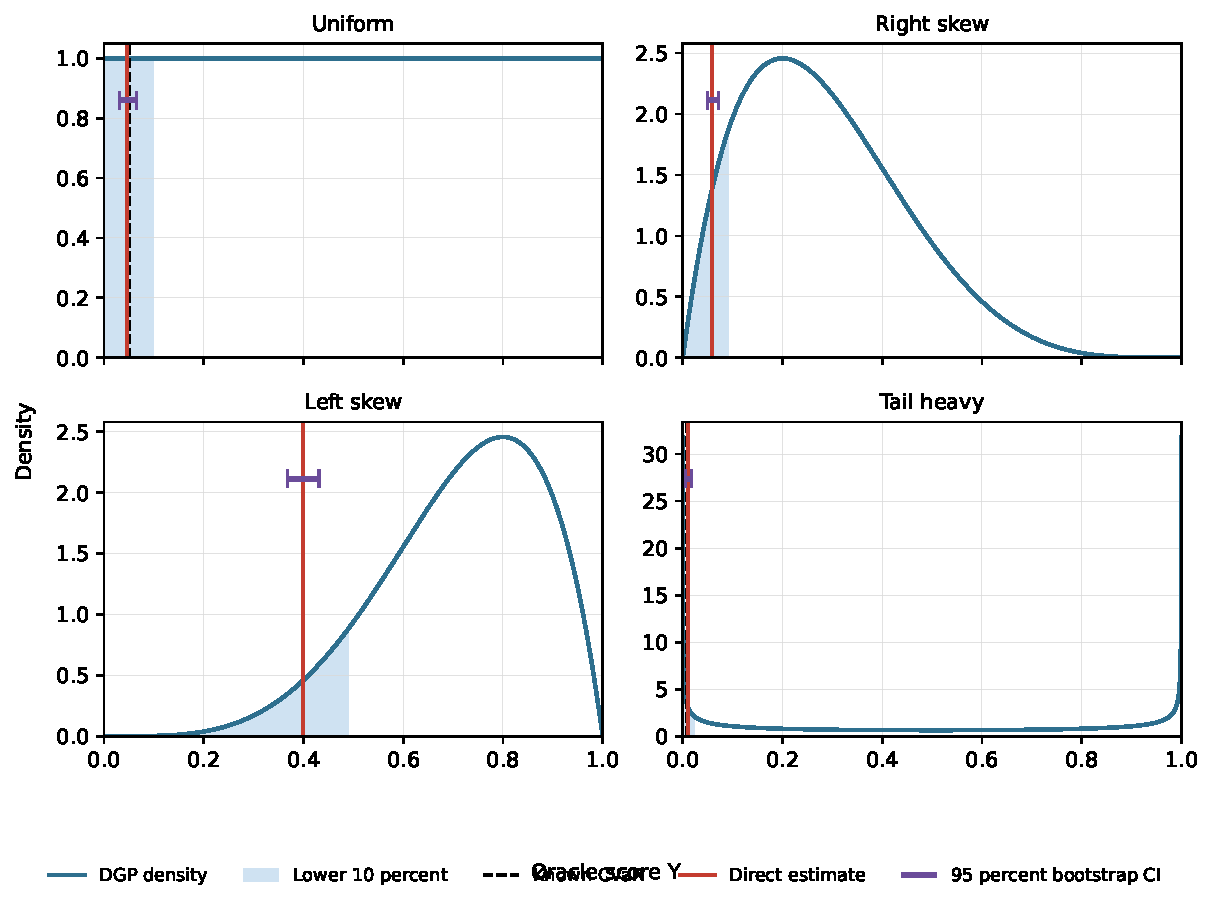
\includegraphics[width=0.92\linewidth]{figures/conclusion_bootstrap_overlay.pdf}
\caption{Representative fixed-seed bootstrap overlay.  The black dashed line is the known DGP CVaR at ten percent.  The red line is one Direct CVaR-CJE estimate.  The horizontal interval is a 95 percent full-refit bootstrap interval that resamples calibration and evaluation rows, refits the cutoff-specific shortfall calibrators, and reselects the cutoff in each bootstrap draw.}
\label{fig-conclusion-bootstrap}
\end{figure}

\section{Testing the CVaR-CJE Pipeline on Arena Dataset}

\subsection{Base-trained calibration applied to target policies}

The first diagnostic asks whether calibration learned on base responses
transports to other policies.  This is a demanding check: the calibration source
is fixed, while the target-policy responses change.

\begin{table}[H]
\centering
\scriptsize
\setlength{\tabcolsep}{4.2pt}
\resizebox{\linewidth}{!}{%
\begin{tabular}{@{}lllrrrll@{}}
\toprule
Policy & Calibration source & Target policy & Full-oracle lower tail & Estimated lower tail & Audit \(p\) & Verdict & Mean check \\
\midrule
base & base & base & 0.2461 & 0.2342 & 0.9540 & Pass & Pass \\
clone & base & clone & 0.2504 & 0.2402 & 0.3206 & Pass & Pass \\
premium & base & premium & 0.2508 & 0.2438 & 0.1756 & Pass & Pass \\
parallel & base & parallel & 0.2591 & 0.2427 & 0.9935 & Pass & Pass \\
unhelpful & base & unhelpful & 0.0000 & 0.0300 & \(<0.001\) & Fails & Fails \\
\bottomrule
\end{tabular}}
\caption{Base-trained transport diagnostic at the bottom-ten-percent target.}
\label{tab-arena-base-trained}
\end{table}

The four main policies pass this transport diagnostic. The unhelpful policy is different: base-trained calibration does
not transport to its unusual outcome distribution, and both the lower-tail check
and the mean check fail.

\subsection{Same-policy recalibration}

The second diagnostic asks what happens when we try to calibrate to a target policy using its own data.

\begin{table}[H]
\centering
\scriptsize
\setlength{\tabcolsep}{4.2pt}
\resizebox{\linewidth}{!}{%
\begin{tabular}{@{}lllrrrll@{}}
\toprule
Policy & Calibration source & Target policy & Full-oracle lower tail & Estimated lower tail & Audit \(p\) & Verdict & Mean check \\
\midrule
base & base & base & 0.2461 & 0.2342 & 0.9540 & Pass & Pass \\
clone & clone & clone & 0.2504 & 0.2724 & 0.0929 & Pass & Pass \\
premium & premium & premium & 0.2508 & 0.2636 & 0.0601 & Pass & Pass \\
parallel & parallel & parallel & 0.2591 & 0.2330 & 0.3334 & Pass & Pass \\
unhelpful & unhelpful & unhelpful & 0.0000 & 0.0000 & 1.0000 & Pass & Pass \\
\bottomrule
\end{tabular}}
\caption{Same-policy recalibration diagnostic at the bottom-ten-percent target.}
\label{tab-arena-same-policy}
\end{table}

Under same-policy recalibration, unhelpful passes.  Its estimated lower-tail
value is exactly zero, matching the full-oracle lower-tail value.  This says the
earlier audit failure, in the previous subsection, was a genuine transport failure.

\begin{figure}[H]
\centering
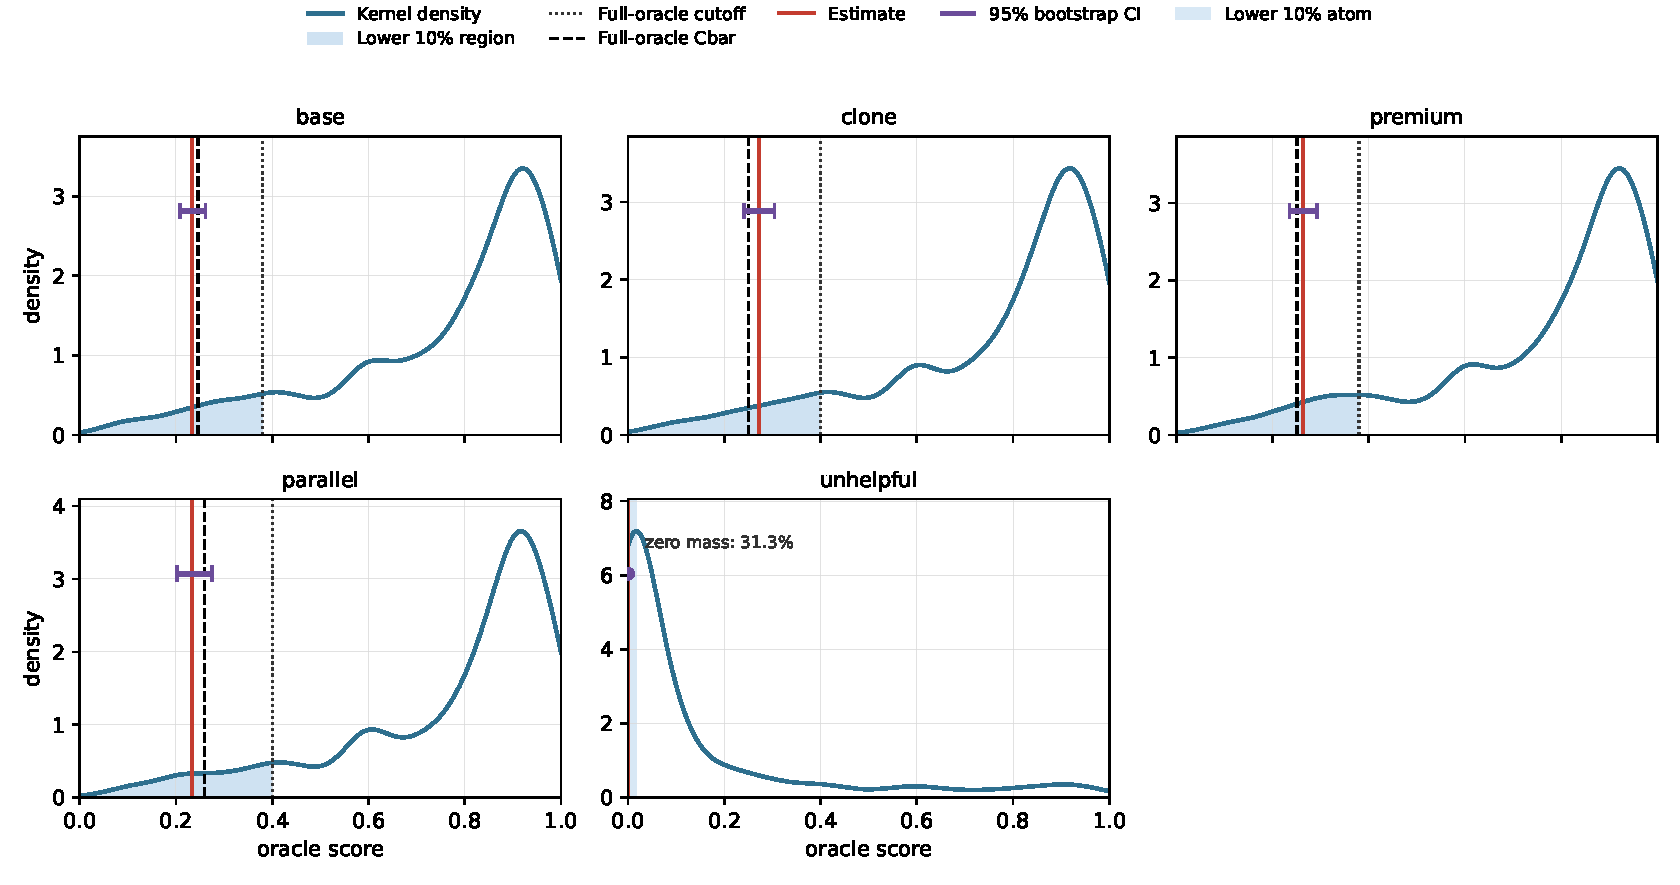
\includegraphics[width=0.7452\linewidth]{figures/arena_density_overlay.pdf}
\caption{Oracle-label densities for the Arena policies.  The dotted line marks the full-oracle ten-percent cutoff, the black dashed line marks the full-oracle lower-tail average, and the red line marks the estimate.  The unhelpful panel shows the mass at zero.}
\label{fig-arena-density-overlay}
\end{figure}


\section{Conclusion}

The synthetic validation study offers positive results.  First, we are able to
recover the mean estimator by setting \(\alpha=1\). Second, the estimator
chooses cutoffs close to the known ten percent quantiles, and estimates ten
percent CVaR with repeated-run averages within 0.0005 of the known CVaR values.
These point-estimation results are unchanged by adding the oracle power
benchmark.  Third, in the transport success case, the audit rejection rate is
close to the five percent target. The audit is therefore
approximately calibrated in this simulation. The Arena test is also encouraging. Base-trained calibration gives us a surrogate model that
transports to the other four main policies, while unhelpful
requires its own calibration because its outcome distribution is unusual.

\end{document}
